\subsection{Mécaniques de jeu}

        \subsubsection{Environement}
            Nous nous sommes beaucoup inspiré du mode multijoueur des premiers Assassin's Creed.
            Nous n'avons pu récréer un système de grimpe car trop ardu à réaliser de nos propres mains.
            En revanche, nous avons réutilisé quelques idées de gameplay pour l'environement, comme les échelles et les portes.\\

            \begin{figure}[hbt!]
                \centering
                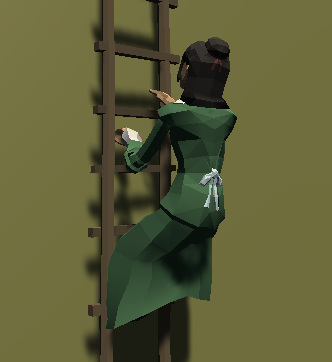
\includegraphics{ladder.png}
                \caption{Joueur grimpant sur l'échelle}
            \end{figure}

            L'échelle permet de créer un peu de verticalité dans nos niveaux.
            Elles ne peuvent être utilisées que par les joueurs,
            prendre de la hauteur permet d'emprunter des raccourcis, mais retire la discrétion (car personne de civilisé devrait être sur les toits !) \\
            
            Les portes peuvent vous permettre de barrer le passage pour échapper à son tueur.
            Elles se ferment quand le joueur passe dessus en courant
            et se réouvrent au bout de quelques secondes.

            \begin{figure}[hbt!]
                \centering
                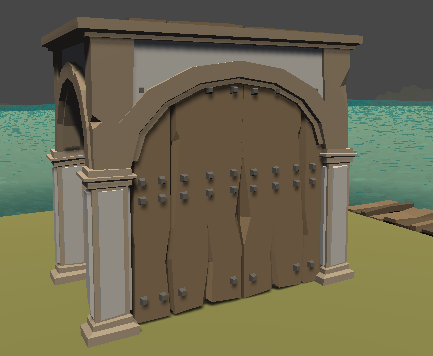
\includegraphics{doors_closed.png}
                \caption{Porte fermée après le passage d'un joueur}
            \end{figure}

        \subsubsection{Déplacement du personnage}
        
            Sans déplacement du personnage, le jeu serait ennuyeux si on ne pouvait interragir avec.
            Nous avons donc réalisé un script de déplacement qui permet au joueur de marcher, courir, sauter\dots\\

            Pour le côté technique, nous avons dans un premier temps utilisé l'Input System de base proposé par Unity. Mais plusieurs problèmes se sont posés:
            \begin{itemize}
                \item On ne peut paramétrer en profondeur les keymaps
                \item Paramétrer d'autres périphériques autre que le clavier/souris est compliqué. Il faudrait avoir des scripts différents pour chaque périphérique, et donc des prefabs différents
            \end{itemize}
            C'est pour cette raison que nous avons migré vers le New Input System.
            Celui ci est ergonomique, multiplateform et permet un mix de différents périphériques à fois, comme la manette par exemple.
            Il a fallu editer certains bout de code pour les rendre compatible; heureusement, la migration ne fut pas très longue après avoir compris son fonctionnement.

            Il est donc actuellement possible de jouer au clavier/souris ou à la manette (pas les deux à fois).
            
        \subsubsection{Attribution des cibles}
            
            C'est Harrys qui a réalisé le script permettant l'attribution des cibles, qui fait usage des méthodes RPC (communication inter-client par l'intermédiaire d'un serveur). Le "MasterClient", un client qui est désigné comme chaque salle pour faire office de maître de jeu, est celui qui désigne la cible de chaque joueur. Il communique ensuite à chacun des clients présent dans la salle sa cible désigné. Cette attribution se fait de façon aléatoire, mais selon certaines règles:
                
                -Un joueur ne peut évidemment pas être sa propre cible
                -Deux joueurs ne peuvent pas être la cible l'un de l'autre
                 Cela permet une plus grande interaction entre les joueurs et pas simplement des scénarios en "1 contre 1".
                -Plusieurs joueurs ne peuvent pas avoir la même cible.
                
            Cependant même si ce script est fonctionnel, il n'a pas encore été implémenté. En somme, l'attribution d'une cible n'a pas encore grande utilité. Le système d'élimination de la cible fera l'objet d'un travail important pour la prochaine soutenance.
        
        
        \subsubsection{Système de verrouilage}

            Le système qui attribue des cibles à chaque joueur n'est pas entièrement implémenté.
            
            Mais le joueur peut vouloir tuer une cible, qu'elle soit la bonne ou non.
            Pour cela, il passe en mode verrouilage, et les personnages pointés par le viseur surbrillent.
            Pour les sélectionner, un coup de molette suffit, et le contour devient alors jaune, pour indiquer que la cible est verouillé.
            Il lui suffit alors d'être à moins d'1 mètre pour l'éliminer.

            \begin{figure}[hbt!]
                \centering
                \begin{subfigure}[b]{0.3\textwidth}
                    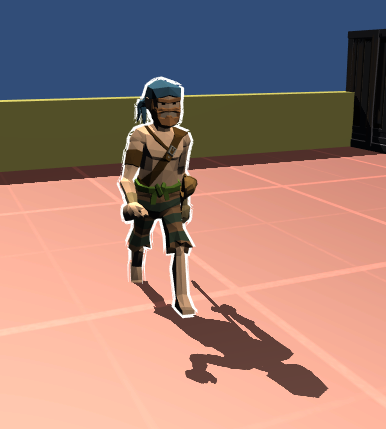
\includegraphics[scale=0.5]{white_outline.png} 
                    \caption{Personnage au centre de l'écran en surbrillance}
                \end{subfigure}
                \hspace{150pt}
                \begin{subfigure}[b]{0.3\textwidth}
                    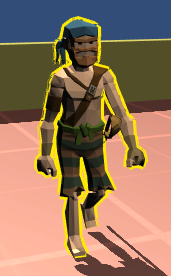
\includegraphics[scale=0.8]{yellow_outline.png} 
                    \caption{Personnage sélectionné et verrouilé}
                \end{subfigure}
                \caption{Système de verrouilage}
            \end{figure}